\documentclass{report}

\input{preamble}
\input{macros}
\input{letterfonts}

\title{\Huge{MAM2000W}\\2LA}
\author{\huge{Alex Cristaudo}}
\date{}

\begin{document}

\maketitle
\newpage% or \cleardoublepage
% \pdfbookmark[<level>]{<title>}{<dest>}
\pdfbookmark[section]{\contentsname}{toc}
\tableofcontents
\pagebreak

\chapter{Eigenvectors, Eigenvalues and Diagonalisation}
\section{Eigenvectors and Eigenvalues}

Reminder:
\dfn{}{
If $A$ is an  $n \times n$ matrix, then a non-zero vector $\mathbf{x}$ is called an eigenvector of $A$ if  $A \mathbf{x} = \lambda \mathbf{x}$ for some scalar $ \lambda $. The scalar is called an eigenvalue of $A$ and  $\mathbf{x}$ is said to be an eigenvector of $A$ corresponding to the eigenvalue  $ \lambda $
}

\mprop{}{
Let $A$ be a square matrix and  $\mathbf{x}$ an eigenvector of $A$ corresponding to eigenvalue  $ \lambda $. Then for every non-zero scalar $ \mu, \mu \mathbf{x}$ is an eigenvector of $A$ corresponding to the eigenvalue of $ \lambda $
}
\begin{myproof}
    We have that $A \mathbf{x} = \lambda \mathbf{x}$. Now $A ( \mu \mathbf{x}) = \mu (A \mathbf{x}) = \mu ( \lambda \mathbf{x}) = \lambda ( \mu \mathbf{x})$
\end{myproof}

\nt{There are infinitely many eigenvectors corresponding to the same eigenvalue}

\thm{}{
\begin{center}
    $ \lambda $ is an eigenvalue of $A \iff \det ( \lambda I - A) = 0$
\end{center}
}
\nt{$\det ( A - \lambda I) = 0 \iff \det ( \lambda I - A) = 0$ so either can be used}

\dfn{}{
Let $A$ be an  $n \times n$ matrix. The determinant $\det ( \lambda I - A)$ is a polynomial of degree $n$ in  $ \lambda $ and is called the characteristic polynomial of $A$. The equation  $ \det ( \lambda I - A) = 0$ is called the characteristic equation of $A$
}

\newpage
\nt{
    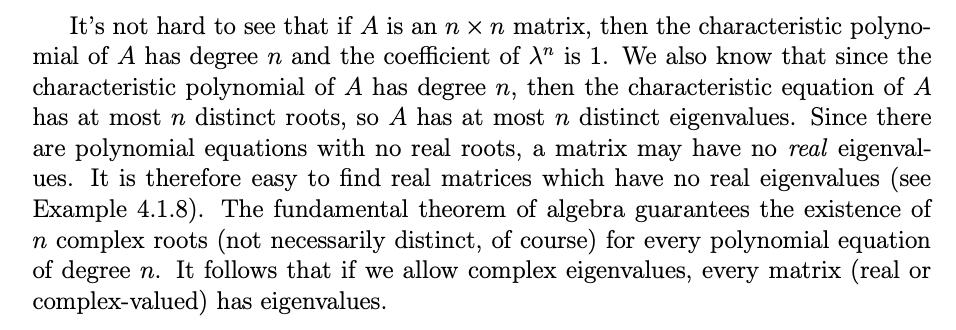
\includegraphics{exp}
}

\ex{}{
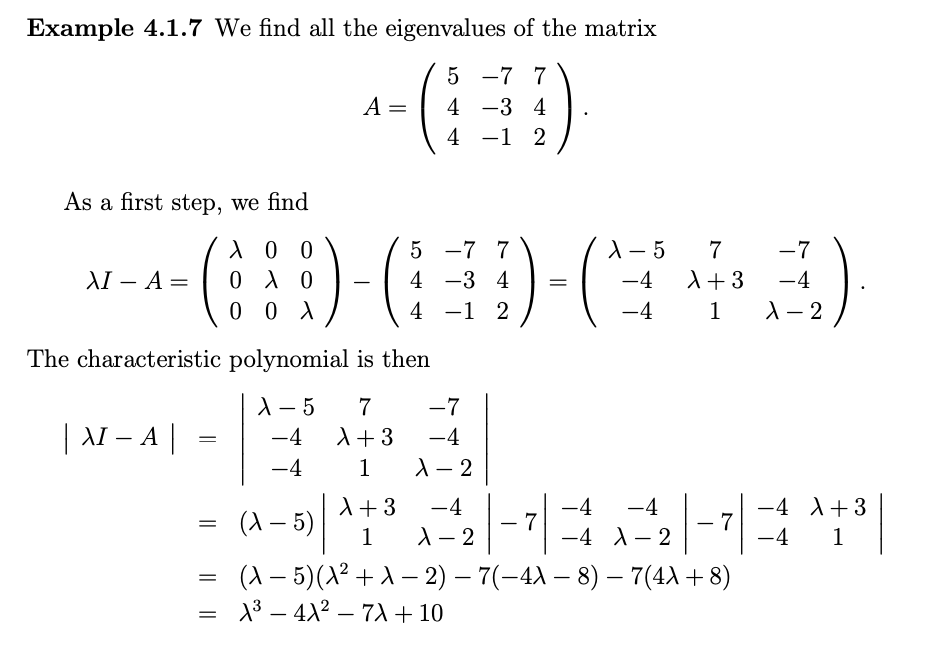
\includegraphics{ex1} }
\ex{}{
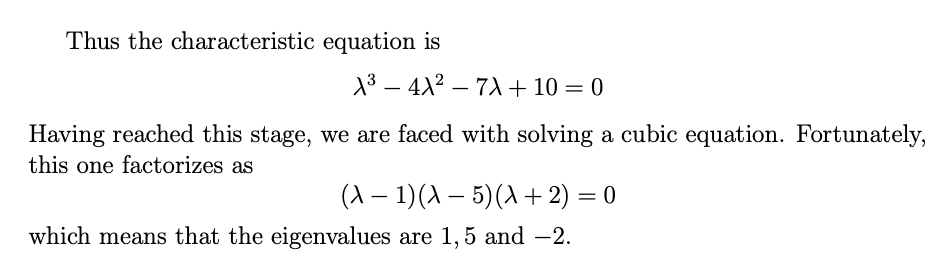
\includegraphics{ex2} }
\ex{}{
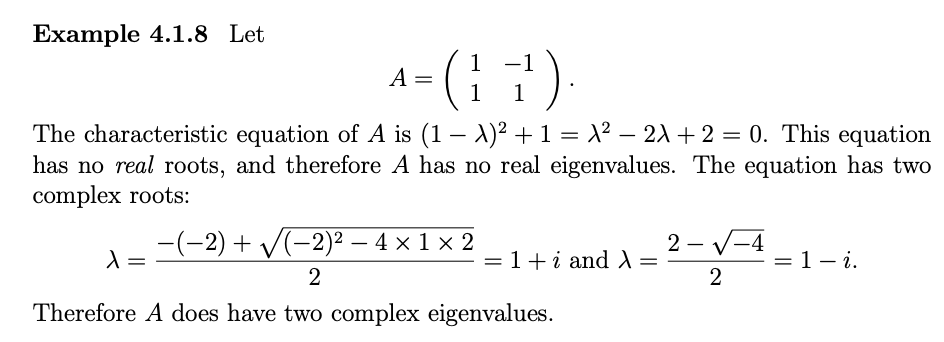
\includegraphics{ex3} }

\thm{}{
Let the eigenvectors of the $n \times n$ matrix of $A$ be  $ \lambda_1, \lambda_2, \cdots, \lambda_{n}$, then
\begin{itemize}
    \item $ \sum \limits _{i=1}^{n} \lambda_i = \sum \limits _{i=1}^{n} a_{ii} $

    \item $\lambda_1 \lambda_2 \cdots \lambda_{n} = \det (A)$
\end{itemize}
}

\begin{myproof}
    We’ll ask you to check these results for 2 ×2 and 3×3 matrices in the exercises. The proof for the general case is similar, but needs properties of determinants
we have not covered
\end{myproof}

\nt{
    Remember $ \sum \limits _{i=1}^{n} a_{ii}$ is known as the trace of the matrix $A$ and denoted by  $ \mathrm{tr}(A)$
}

\thm{}{
Let $ \lambda $ be an eigenvalue of the $n \times n$ matrix $A$. The eigenvectors of  $A$ associated with  $ \lambda $ are the non-zero vectors in $NS( \lambda I-A)$ and hence together with the zero vector, form a subspace of $\mathbb{R}^n$ (or $\mathbb{C}^n$ if $A$ is complex)
}
\begin{myproof} TODO: \\
    An important fact that we see almost immediately is that
the eigenvectors associated with an eigenvalue "almost" form a vector subspace. To
see this, suppose that $ \lambda $ is an eigenvalue of A. A non-zero eigenvector x, associated
with $ \lambda $, is a solution of the equation ($ \lambda I - A$)x = 0. This means that it is a member
of the nullspace of $ \lambda I - A$. Moreover, all members of this nullspace, except the zero
vector, are eigenvectors corresponding to the eigenvalue $ \lambda $
\end{myproof}

\dfn{}{
    Let $A$ and  $ \lambda $ be as in the above theorem. Then $NS( \lambda I-A)$ is called the eigenspace associated with $ \lambda $. We use notation $W_{ \lambda }$ for this eigenspace
}
\nt{We include $\mathbf{0}$ in the eigenspace as it is part of the nullspace (but not eigenvectors)}

\ex{}{
    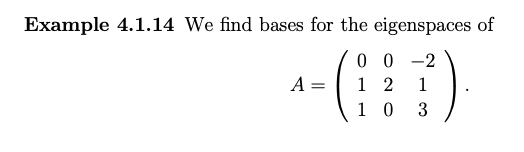
\includegraphics{ex4}
    ~\\
    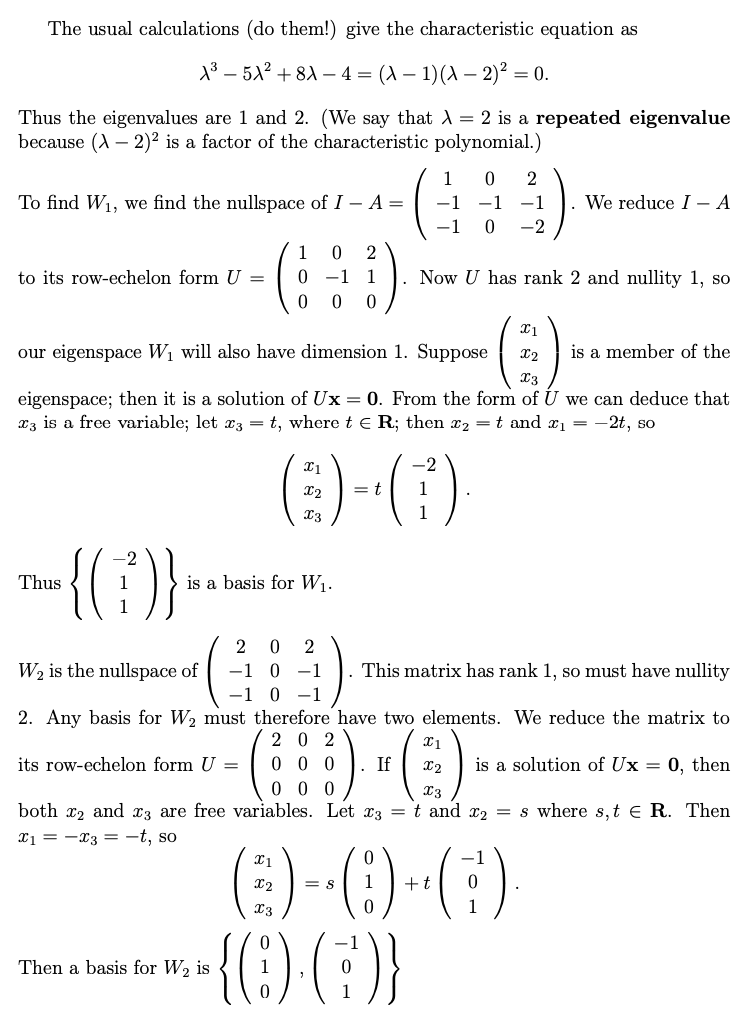
\includegraphics{ex5}
}
\ex{}{
    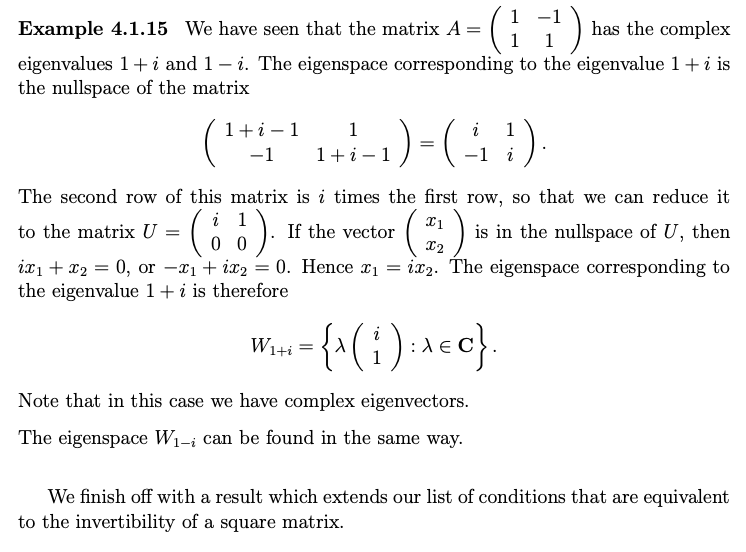
\includegraphics{ex6}
}

\thm{}{
An $ n \times n$ matrix $A$ is invertible if and only if  $ \lambda = 0$ is not an eigenvalue of $A$
}
\begin{myproof}
    If $ \lambda = 0$ is an eigenvalue, then $ 0 = \det ( \lambda I - A) = \det (-A) = (-1)^n \det (A) \implies \det (A) = 0 \implies A$ is not invertible. The converse is similar  
\end{myproof}

\section{Diagonalization}

\thm{}{
    Let $A$ be an  $n \times n $ matrix
    \begin{itemize}
        \item If $A$ has  $n$ linearly independent eigenvectors  $ \mathbf{v}_1, \mathbf{v}_2, \cdots, \mathbf{v}_{n}$ and $P$ is the matrix whose  $j$th column is  $\mathbf{v}_j$, then $P^{-1}AP$ is a diagonal matrix  $D$ and the entries  $d_{jj}$ (on the main diagonal of  $D$) are exactly the eigenvalues corresponding to the eigenvectors  $\mathbf{v}_j$
        \item If there is an invertible matrix $P$ such that $P^{-1}AP$ is a diagonal matrix  $D = (d_{ij})$, then for each  $j$, the  $j$th column of $P$ is an eigenvector of  $A$ corresponding to the eigenvalue  $D_{jj}$ and hence  $A$ has  $n$ linearly independent eigenvectors
    \end{itemize}
}

\begin{myproof}[]
    \begin{itemize}
        \item $P$ is square and has rank  $n$ since its columns are linearly independent. Now we calculate  $AP$ one column at a time: \\
             \[
            \begin{aligned}
                j \text{th column of } AP  & = A\left( j \text{th column of} P \right) \\
                 & = A\mathbf{v}_j \\
                 & = \lambda _j \mathbf{v}_j \left( \text{Dfn for eigenvectors and values }   \right) 
            \end{aligned}
            \]
        Now we calculate $PD$ once column at a time \\
         \[
        \begin{aligned}
            j\text{th column of } PD  & = P\left( j\text{th column of } D \right) \\
             & = P \begin{pmatrix} 0 \\ \vdots  \\ \lambda _j  \\ \vdots  \\ 0 \end{pmatrix} \\
              & = \lambda _j \mathbf{v}_j
        \end{aligned}
        \]
        So $AP = PD$ and thus  $P^{-1}AP = D$
        \nt{We know $P^{-1}$ exists because  $ \mathrm{Rank}(P) = n$

        Also we have that $A = PDP^{-1}$} 
    \item If $P^{-1}AP = D$, then  $AP=PD$. Let  $\mathbf{v}_j$ be the $j$th column of  $P$. Then comparing  $j$th columns on each side of the equation  $AP=DP$, we see that  $A \mathbf{v}_j = d_{jj}\mathbf{v}_j$. Hence $\mathbf{v}_j$ is an eigenvector of $A$ corresponding to eigenvalue  $d_{jj}$. Since  $P$ is invertible, it must have rank  $n$ and thus the columns of  $P$ must be linearly independent
    \end{itemize}
\end{myproof}

\ex{}{
Let $A = \begin{pmatrix} 0 & 0 & -2 \\ 1 & 2 & 1 \\ 1 & 0 & 3 \end{pmatrix}.  $ This has characteristic equation $\left( \lambda -1 \right)\left( \lambda -2 \right)^2 = 0  $

The eigenspaces follow from this and we get: \\
$W_2$ has basis  $\{ \begin{pmatrix} -1 \\ 0 \\ 1 \end{pmatrix}, \begin{pmatrix} 0 \\ 1 \\ 0 \end{pmatrix}   \} \\ W_1$ has basis $\{ \begin{pmatrix} -2 \\ 1 \\1 \end{pmatrix}  \}$ \\ The three vectors are linearly independent so we can form the matrix $P = \begin{pmatrix} -1  & 0 & -2 \\ 0  & 1 & 1 \\ 1 & 0 & 1 \end{pmatrix} $ which has as columns the 3 eigenvectors. \\ Now  $P^{-1} = \begin{pmatrix} 1 & 0 & 2 \\ 1 & 1 & 1 \\ -1 & 0 & -1 \end{pmatrix} $ and thus $P^{-1}AP = \begin{pmatrix} 2 & 0 & 0 \\ 0 & 2 & 0 \\ 0 & 0 & 1 \end{pmatrix} $
\nt{Notice that there is no preferred order for writing down the eigenvectors of A as
columns of P. Once you have decided on the order though, the matrix D will have
eigenvalues on the diagonal in the order that you wrote down the eigenvectors in P.
This means that you can diagonalize A in different ways, depending on the order in
which you do things. This is not a problem as long as you remember to write down
eigenvectors and eigenvalues in the same order}
\nt{We do not need all eigenvalues to be distinct just the eigenvectors in the eigenspaces}
}

\dfn{}{
    We say a square matrix $A$ is diagonalizable if there is an invertible matrix  $P$ such that  $P^{-1}AP = D$ where  $D$ is a diagonal matrix.  $P$ is said to diagonalize  $A$
}

\thm{}{
    \[
    \begin{aligned}    
        A \text{ is diagonalizable } &  \iff A \text{ has } n \text{ linearly independent eigenvectors } \\
                                     & \iff \mathbb{R}^n \text{ has a basis consisting of eigenvectors of } A
    \end{aligned}
    \]
}

\nt{
    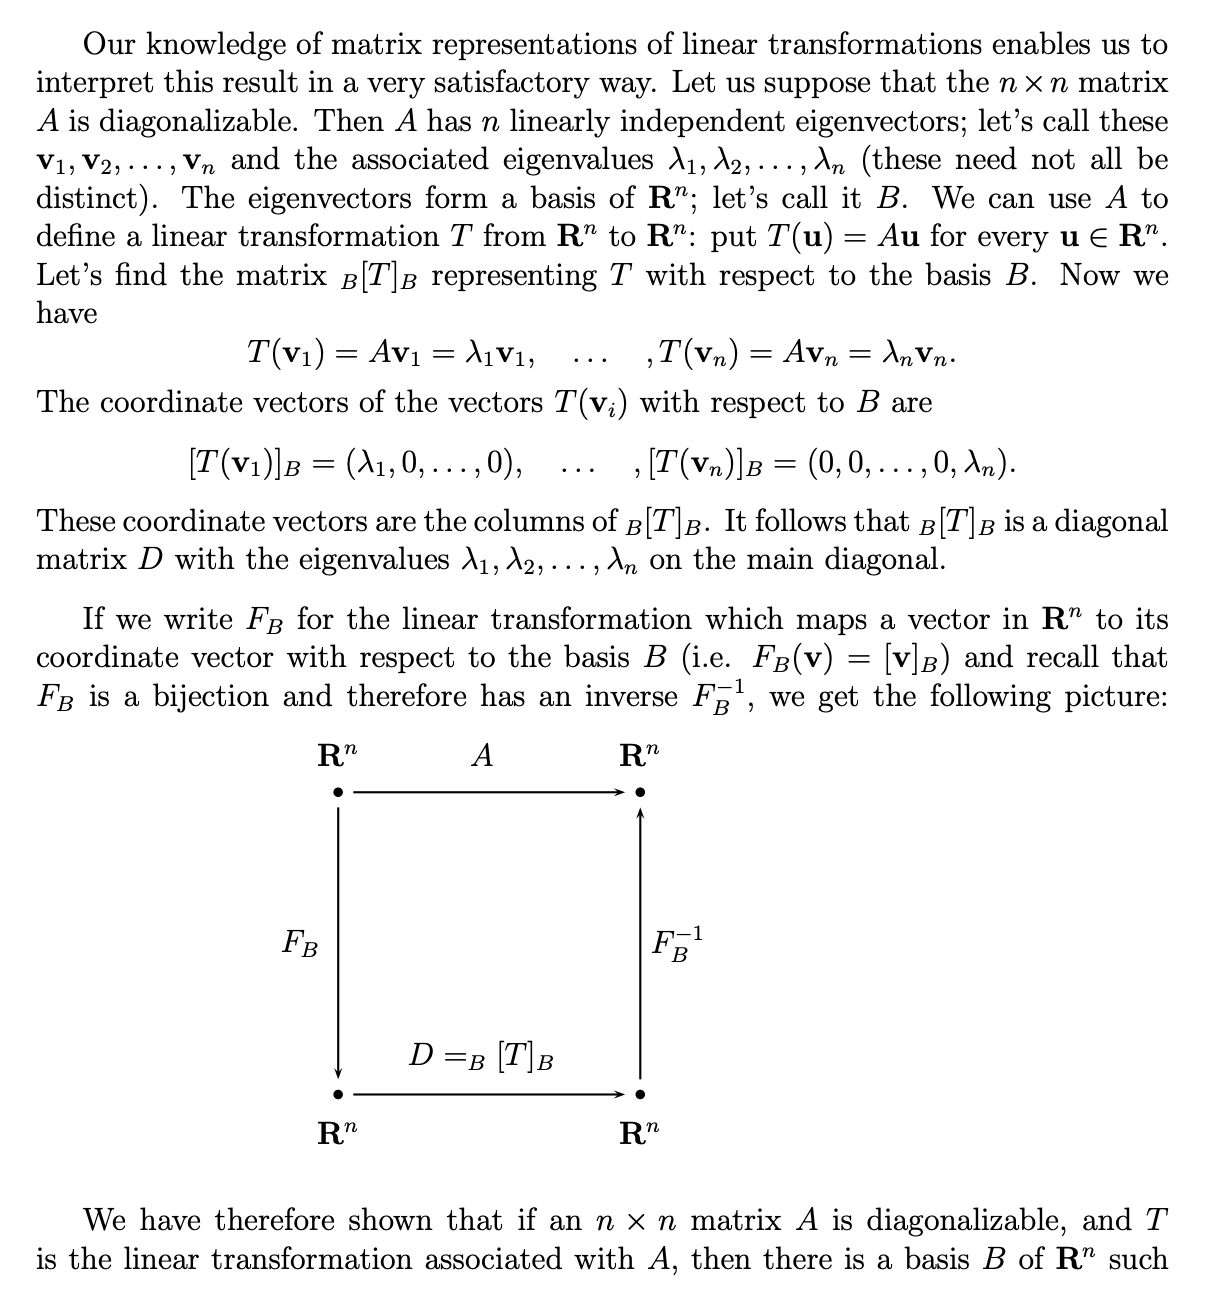
\includegraphics[scale = 0.8]{nt1}
    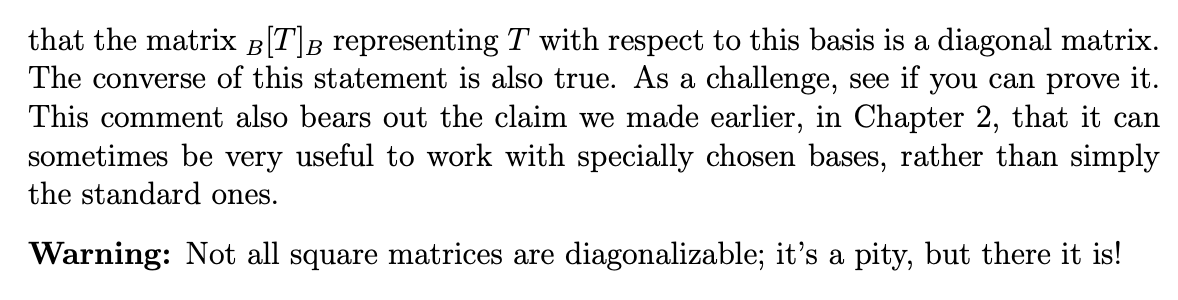
\includegraphics[scale = 0.8]{nt2}
}

\nt{A sufficient condition for this is $n$ distinct eigenvalues}

\thm{}{
    Let $ \mathbf{v}_1, \mathbf{v}_2, \cdots, \mathbf{v}_{m}$ eigenvectors of $A$ associated with distinct eigenvalues $ \lambda_1, \lambda_2, \cdots, \lambda_{m}$. Then $\{ \mathbf{v}_1, \mathbf{v}_2, \cdots, \mathbf{v}_{m} \}$ are linearly independent.
}
\begin{myproof}[]
    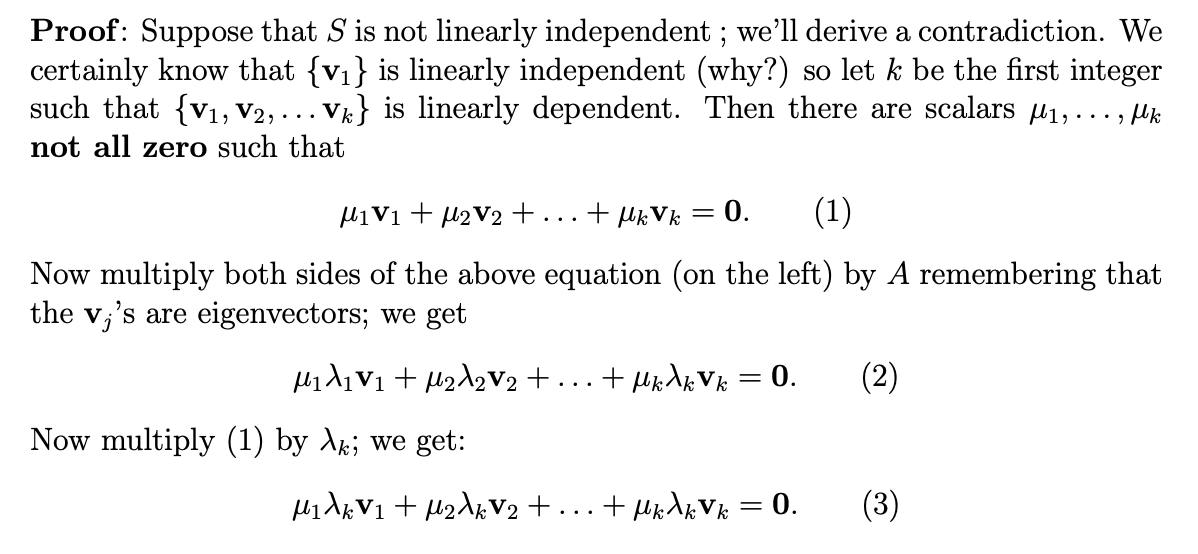
\includegraphics[scale = 0.7]{prf1} \\
    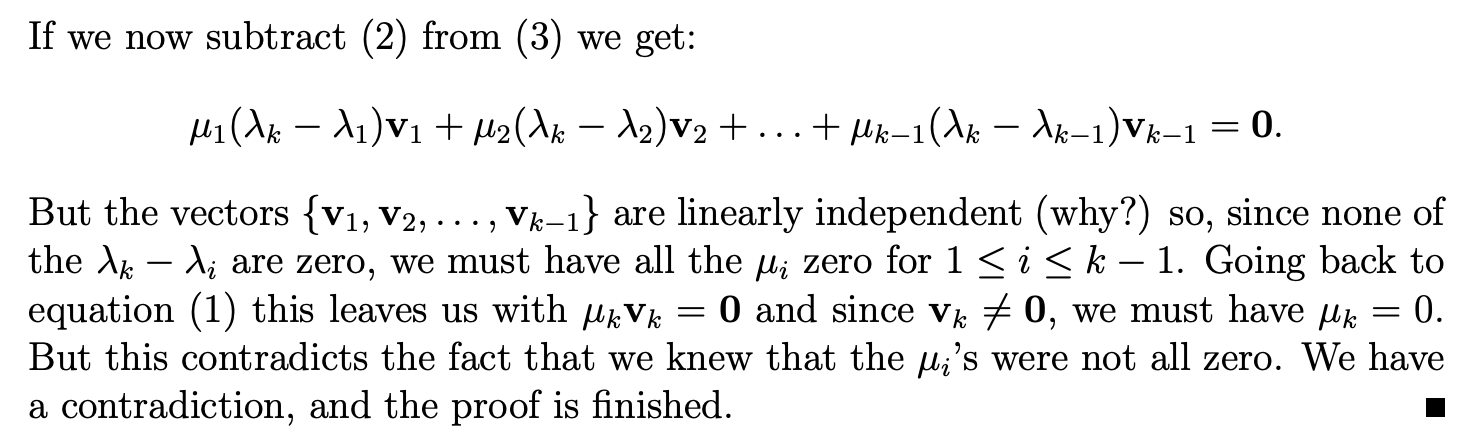
\includegraphics[scale = 0.7]{prf2}
\end{myproof}

\nt{
Given $n \times n$ matrix
\begin{enumerate}
    \item Determine eigenvalues \\ If you find $n$ distinct eigenvalues, then you can diagonalize
    \item Otherwise (repeated eigenvalues), it is still possible to diagonalize the matrix
\end{enumerate}
}
\ex{}{
For $A = \begin{pmatrix} 0 & 0 & -2 \\ 1 & 2 & 1 \\ 1 & 0 & 3 \end{pmatrix} $ gives characteristic equation $(1- \lambda )(2- \lambda )^2 = 0$
\\ In this case we say $2$ has algebraic multiplicity  $2$. \\ Remember as a check, sum of eigenvalues is sum of diagonal entries (double counting 2 in this case) \\
$W_1 \{ s \begin{pmatrix} -2 \\ 1 \\ 1 \end{pmatrix}: s \in \mathbb{R} \}$ \\ $W_2 = \{ s \begin{pmatrix} -1 \\ 0 \\ 1 \end{pmatrix} +t \begin{pmatrix} 0 \\ 1 \\ 0 \end{pmatrix} : s,t \in \mathbb{R}  \}$ (we say eigenvalue $2$ has geometric multiplicity  $2$)
\\ $P = \begin{pmatrix} -2  & -1 & 0 \\ 1 & 0 & 1 \\ 1 & 1 & 0 \end{pmatrix} $ (if geometric multiplicity = algebraic, fine. Geometric multiplicity must always be less than or equal to algebraic multiplicity
}

\ex{}{
$\begin{pmatrix} 1 & 2 \\ 0 & 1 \end{pmatrix}  \Longrightarrow \lambda = 1, \lambda = 1$ (triangular matrix) with algebraic multiplicity $2 \ \ \left( (1- \lambda )(1- \lambda )=0 \right) $
    \\ $W_1 = NS \begin{pmatrix} 0  & 2 \\ 0 & 0 \end{pmatrix} $. We have that $ \mathrm{Nullity} = 1 \implies $ geometric multiplicity of $1$ is  $1$, hence not diagonalizable
}

\ex{}{
    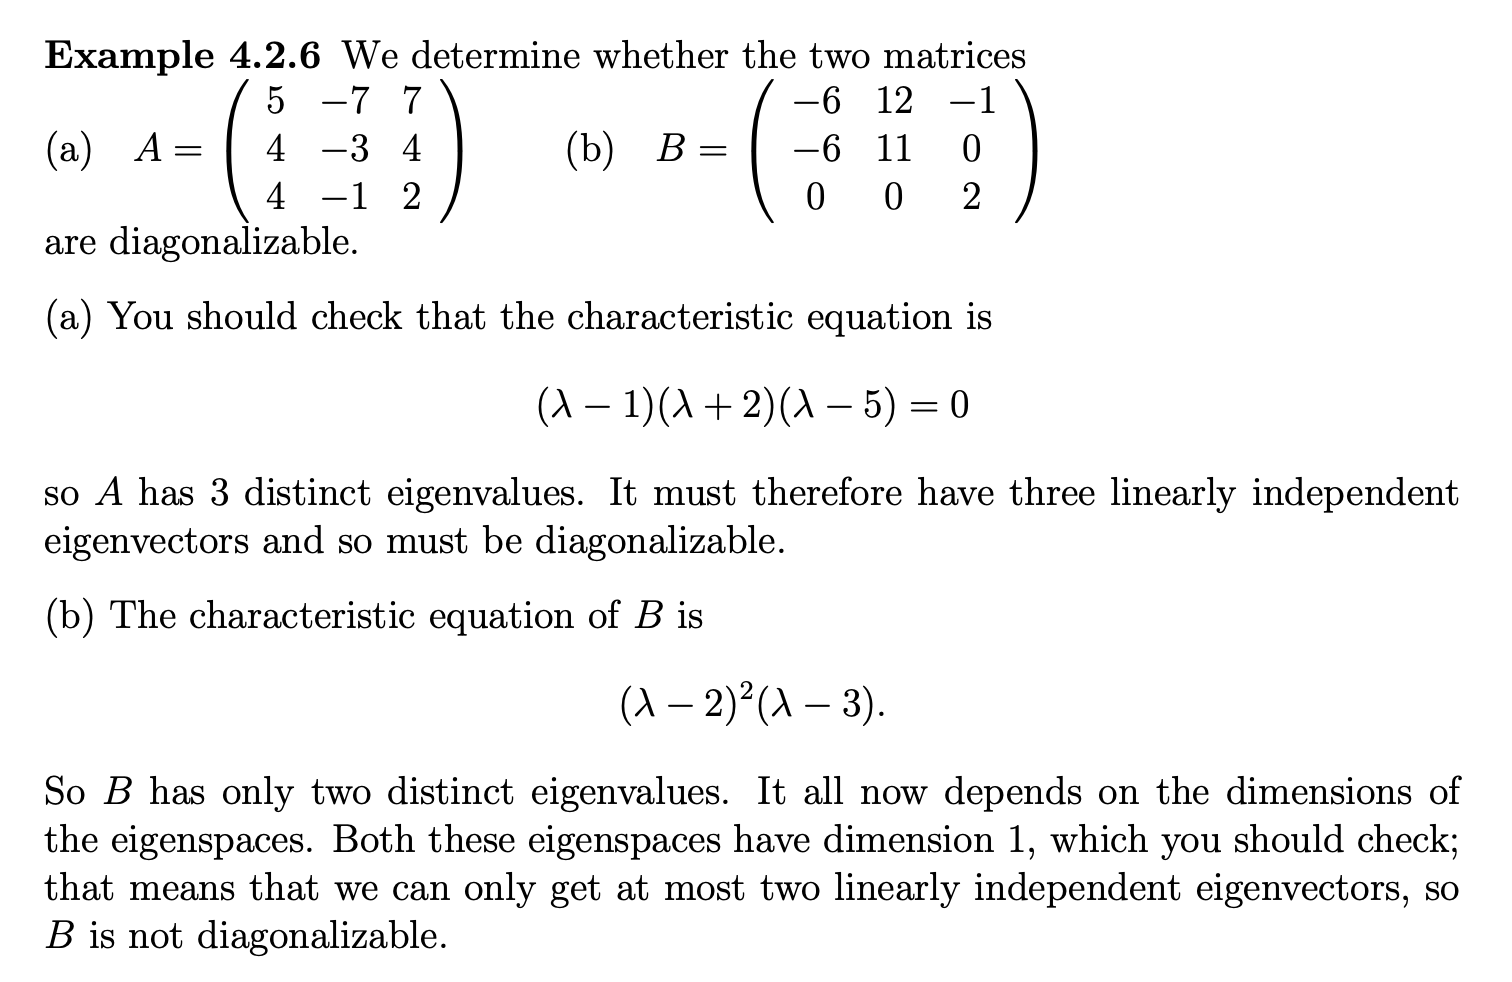
\includegraphics[scale = 0.6]{ex7}
}

\section{Applications of Diagonalization}
\textbf{Markov Matrices} \\
Recall that in Example 1.1.1 we set up a matrix which described, in terms
of percentages, what happened each month to the transport preferences of UCT
students commuting to campus. The matrix was
\\$M = \begin{pmatrix} 0.8 & 0.1 \\ 0.2 & 0.9 \end{pmatrix} $ \\
This is an example of a stochastic, Markov, or probability matrix. We give the
general definition now.

\dfn{}{
    A square matrix $M - (m_{ij})$ is called a Markov Matrix if 
     \begin{itemize}
         \item $m_{ij} \ge 0$ for all  $i$ and  $j$
         \item for each  $j$,  $m_{1j} + m_{2j} + \ldots + m_{kj} = 1$ \\ (the entries in each column add up to 1)
    \end{itemize}
}
\nt{These are also called transition matrices}

Lets look at some examples where diagonalizing a matrix is useful:

\ex{}{
 Let’s make the following
assumptions about UCT students and their transport preferences:
\begin{itemize}
    \item Ten thousand students have to get to the UCT campus every day; this number
stays constant.
\item At the start of each month, 20\% of students who were using the Jammie
Shuttle change to using their own transport and 10\% of students using their
own transport change to using the Jammie Shuttle.
\item At the beginning of the first month of the academic year, 6000 students use
the Jammie Shuttle
\end{itemize}
We want to explore the way in which the transport preferences will change with
time, and what the long term trend (if any) will be
\\ First let us denote $x(n)$ as the number of students using the Jammie at the beginning of month  $n$ \\  $y(n)$ is the number of students using their own transports
\\ This means that \\
 \[
\begin{aligned}
    x(n+1)  & = 0.8x(n) + 0.1y(n) \\ y(n+1)  & = 0.9y(n) + 0.2x(n)
\end{aligned}
\]
So we have that: \\
\begin{center}
    $ \begin{pmatrix} 0.8 & 0.1 \\ 0.2 & 0.9 \end{pmatrix} \begin{pmatrix} x(n) \\ y(n) \end{pmatrix} = \begin{pmatrix} x(n+1) \\ y(n+1) \end{pmatrix}  $ 
    At the beginning of month $2$: \\
     \begin{center}
        $\begin{pmatrix} 0.8  & 0.1 \\ 0.2  & 0.9 \end{pmatrix} \begin{pmatrix} 6 \\ 4 \end{pmatrix}  = \begin{pmatrix} 5.2 \\ 4.8 \end{pmatrix} $ \\ so there will be 5200 Jammie users and 4800 using their own transport
    \end{center}
    but now we can get general formula $ \begin{pmatrix} x(n) \\ y_(n) \end{pmatrix} = \begin{pmatrix}  0.8 & 0.1 \\ 0.2 & 0.9 \end{pmatrix}^n \begin{pmatrix} x(0) \\ y(0) \end{pmatrix} =   \begin{pmatrix}  0.8 & 0.1 \\ 0.2 & 0.9 \end{pmatrix}^n \begin{pmatrix} 6000 \\ 4000 \end{pmatrix}  $
    \\ Now if we diagonalize some matrix $A = SDS^{-1}$ (if  $D = S^{-1}AS \implies A = SDS^{-1}$), then $A^n = (SDS^{-1})^n 
    = \underbrace{SDS^{-1}SDS^{-1} \ldots SDS^{-1}}_\text{$n$ times} = SD^nS^{-1}$ \\ Now for $ D = \begin{pmatrix}
    d_{11}  & 0  & \cdots  & 0 \\
    0  & d_{22}  & \cdots  & 0 \\
    \vdots & \vdots & \ddots & \vdots \\
    0  & 0  & \cdots & d_{mm}
    \end{pmatrix} $, we get that \\ $D^n = \begin{pmatrix}
    d_{11}^n  & 0  & \cdots  & 0 \\
    0  & d_{22}^n  & \cdots  & 0 \\
    \vdots & \vdots & \ddots & \vdots \\
    0  & 0  & \cdots & d_{mm}^n
    \end{pmatrix}$  



\end{center}
and we use this to calculate $A^n$
The steady-state vector is one where $\begin{pmatrix} x(n+1) \\ y(n+1) \end{pmatrix} = \begin{pmatrix} x(n) \\ y(n) \end{pmatrix} $, that is, we take $n \to \infty $ and get the matrix the state tends towards
}

\ex{}{Differential equation example}

\end{document}
